\chapter{Introduction}
\label{chap:intro}
The demand for electricity continues to grow as the world develops. To fulfill the demand, the electrical grid must expand. The reduce the effects of climate change, green energies are being sought after more than ever. Green energy, however, is often generated with an offset to the demand \cite{Mertens_2022}. Solar energy peaks in the day, whereas electricity demand peaks in the mornings and afternoons. Wind energy is also very inconsistent, having strong peaks and troughs as the day progresses \cite{Ernst_1999}. It is often the job of coal or gas power plants to supplement the energy demands and keep the grid stable. 

To negate the negative outcomes of green energy, the energy can be stored to dampen the transient effects and ensure power is available when it is required. Chemical batteries can be used for this, but are too expensive to be applied large scale, and the process of mining for the materials required also has negative effects on the climate. Phase change materials (PCMs) are a promising alternative that can be applied large scale to store energy as heat \cite{Datas_López-Ceballos_López_Ramos_del_Cañizo_2022}.

As the material melts, the temperature is kept at a near-constant temperature. This also makes them very good candidates for a thermal management system. In spacecraft structures, for example, many extreme temperature cycles can occur as a satellite orbits the Earth \cite{Gordo_Frederico_Melicio_Duzellier_Amorim_2020}. PCMs can help to keep electrical components' temperatures constant to improve their performance.

PCMs on their own, however, suffer many issues. The main problem is that they generally have very low thermal conductivity \cite{Reza_Vakhshouri_2020}. This means that the PCM only melts in the region near a heat source, which gives rise to a high temperature gradient throughout the domain. This means the latent heat effects of the PCM are not recognized. Work has been conducted \cite{Xu_Zhang_Fang_2022} to improve the thermal conductivity of a PCM, but the most promising option is to use lattice structures.

Lattice structures themself are only a viable option thanks to advances in additive manufacturing technology. Additive manufacturing allows small-scale production of complex parts that were previously either impossible or too difficult to produce. Lattice structures can now be created without the need for complex single-use molds for casting. Additive manufacturing also allows for the production of complex topologically optimized thermal and structural parts.

\pagebreak
\begin{figure}[ht]
    \centering
    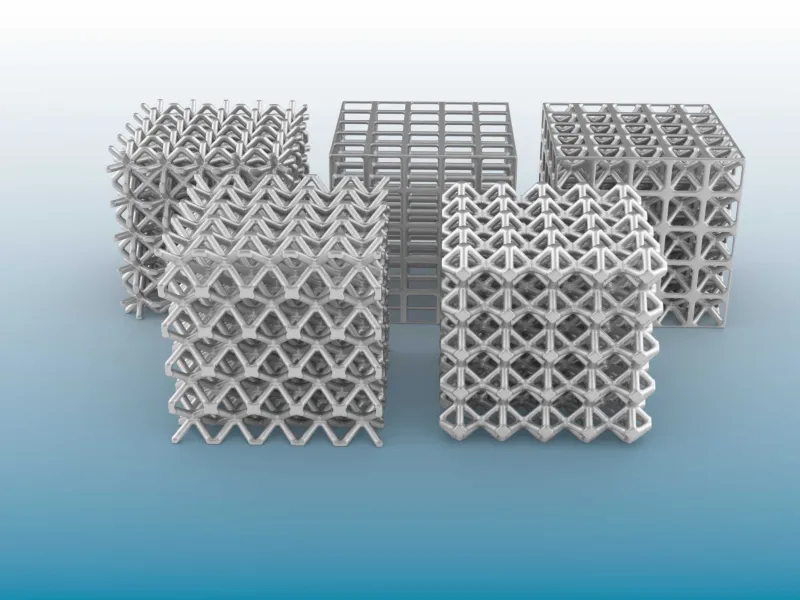
\includegraphics[width=0.7\linewidth]{figures/chapter_1/LatticeStructures.png}
    \caption{Example of lattice structures with various unit cells \cite{Gen3DAdmin_2021}}
\end{figure}

Schirp-Schoenen, \cite{Schirp_2020} showed that the effective thermal conductivity of a PCM can be significantly increased using lattice structures, even when the volume fraction of the lattice is low. More unit cells were later investigated by Soika, et al., \cite{Piacquadio_Soika_Schirp_Schröder_Filippeschi_2023} and semi-analytical formula for the effective material properties were developed. Homogenized models for the effective structural properties of the unit cells have also been by \cite{Bühring_Soika_Schirp-Schoenen_Schröder_2022}. 

This thesis begins by introducing the fundamental theoretical basis of all the topics involved. Those are the theory of heat transfer, the Stefan problem, structural mechanics and optimization methods. Following that, the state of the art is investigated to ensure a good practical basis of the problem is understood. Topology optimization and multi-functional topology optimization are the most important topics investigated in this thesis, and many methods have been developed for both. This thesis tries to utilize and adapt those methods to the current problem.

With the theory and state-of-the-art understanding, the single-functional topology optimization problems are implemented using the finite element method. These include structural, thermal and phase change topology optimization. The results are briefly discussed before moving on to the multi-functional topology optimization implementation. Finally, some test cases are produced to ensure the solver can find optimums given different boundary conditions.